\documentclass[11pt,a4paper]{article}

\usepackage[utf8]{inputenc}
\usepackage[T1]{fontenc}
\usepackage{lmodern}
\usepackage{microtype}
\usepackage[a4paper, margin=0.7in, top=0.7in, bottom=0.7in]{geometry}
\usepackage{amsmath,amssymb}
\usepackage{booktabs}
\usepackage{tabularx}
\usepackage{graphicx}
\usepackage{xcolor}
\usepackage{hyperref}
\usepackage{fancyhdr}
\usepackage{pgfplots}
\usepackage{tikz}
\usepackage{listings}
\usepackage{float}
\usepackage{enumitem}
\usepackage{lastpage}
\usepackage{titlesec}

\titlespacing*{\section}{0pt}{7pt plus 1.5pt minus 1.5pt}{3pt plus 1pt minus 1pt}
\titlespacing*{\subsection}{0pt}{5pt plus 1pt minus 1pt}{2.5pt plus 0.5pt minus 0.5pt}

\pgfplotsset{compat=1.18}
\setlist{noitemsep, topsep=1pt, parsep=0.5pt, partopsep=0pt}

% Color definitions
\definecolor{primaryblue}{RGB}{20, 50, 110}
\definecolor{accentblue}{RGB}{41, 128, 185}
\definecolor{darkgray}{RGB}{45, 45, 45}
\definecolor{lightgray}{RGB}{246, 248, 250}
\definecolor{bordergray}{RGB}{210, 215, 225}

\hypersetup{
    colorlinks=true,
    linkcolor=primaryblue,
    citecolor=primaryblue,
    urlcolor=accentblue
}

% Header and Footer configuration
\pagestyle{fancy}
\fancyhf{}
\rhead{\small \textcolor{darkgray}{CMPE 344 -- Prelab 2 Report}}
\lhead{\small \textcolor{darkgray}{Group: FF78\_G17}}
\rfoot{\small Page \thepage\ of \pageref{LastPage}}
\renewcommand{\headrulewidth}{0.5pt}
\renewcommand{\footrulewidth}{0.3pt}

\begin{document}

% =========================================================================
% PAGE 1: TITLE, INTRODUCTION, EXPERIMENTAL SETUP
% =========================================================================

\begin{center}
    {\LARGE \textbf{\textcolor{primaryblue}{BO\u{G}AZ\.{I}\c{C}\.{I} UNIVERSITY}}}\\[0.2em]
    {\large \textbf{Department of Computer Engineering}}\\[0.45em]
    {\Large \textbf{CMPE 344: Computer Organization}}\\[0.25em]
    {\large \textbf{Fall 2026 -- Prelab 2 Report}}\\[0.7em]
    \rule{\textwidth}{1.1pt}\\[0.5em]
    {\huge \textbf{Benchmarking Processor Designs with CoreMark}}\\[0.3em]
    {\large Workload Profiling, Compiler Optimization Analysis, and RISC-V ISA Extensions}\\[0.5em]
    \rule{\textwidth}{1.1pt}\\[0.7em]
\end{center}

\begin{table}[H]
\centering
\begin{tabularx}{\textwidth}{lX r}
    \textbf{Group ID:} & \textbf{FF78\_G17} & \textbf{Course:} CMPE 344: Computer Organization \\
    \textbf{Target Platform:} & Apple M2 (Host) / CORE-V Wally (Lab 2) & \textbf{Benchmark:} EEMBC CoreMark v1.0 \\
\end{tabularx}
\end{table}

\vspace{-0.3em}

\section{Introduction and Objectives}
In embedded systems and Internet of Things (IoT) hardware development, selecting the optimal processor core is a central architectural decision that balances computational throughput, silicon footprint, dynamic power dissipation, and code density. When physical silicon prototyping across candidate architectures is cost-prohibitive, software-driven architecture benchmarking offers empirical guidance.

The \textbf{Embedded Microprocessor Benchmark Consortium (EEMBC)} introduced CoreMark as an industry-standard, synthetic yet realistic processor benchmark tailored specifically for embedded and general-purpose CPU cores. Unlike legacy benchmarks such as Dhrystone---which suffer from compiler over-optimization, unrealistic string manipulation, and standard library dependencies (\texttt{printf}, \texttt{malloc})---CoreMark isolates fundamental integer CPU pipeline performance through carefully bounded, deterministic algorithms.

This prelab establishes the empirical foundation for upcoming architectural evaluations on the configurable \textbf{CORE-V Wally RISC-V processor} (Lab 2). In this report, we:
\begin{enumerate}[leftmargin=1.4em]
    \item Measure CoreMark throughput (\texttt{Iterations/Sec}) on the host system across compiler optimization levels (\texttt{-O0}, \texttt{-O1}, \texttt{-O2}, \texttt{-O3}, \texttt{-Ofast}, \texttt{-march=native}), and report the actual clock frequency.
    \item Provide a thorough technical explanation of the key algorithms implemented in CoreMark.
    \item Describe the architectural specifications, instruction formats, and hardware trade-offs of five target RISC-V ISA extensions: \textbf{RV32I}, \textbf{RV32IM}, \textbf{RV32IMC}, \textbf{RV32GC}, and \textbf{RV64I}.
\end{enumerate}

\section{Experimental Setup and System Architecture}
As mandated by the assignment guidelines, all benchmark runs were conducted directly on the host system without virtualization or container overhead to ensure direct, unmediated hardware access.

\subsection{Hardware Specifications and Clock Frequency Analysis}
System introspection utilities were employed to extract microarchitectural topology. On Linux systems, \texttt{lscpu} displays processor architecture; on macOS Darwin, equivalent information was acquired via \texttt{system\_profiler SPHardwareDataType} and kernel hardware MIBs via \texttt{sysctl}:
\begin{itemize}[leftmargin=1.4em]
    \item \textbf{System Model:} Apple MacBook Air (Model Identifier: \texttt{Mac14,2}, Apple Silicon).
    \item \textbf{CPU Microarchitecture:} Apple M2 (ARMv8.5-A 64-bit architecture, 8-wide decode out-of-order execution core).
    \item \textbf{Core Topology and Heterogeneity:} 8 total physical cores in an asymmetric big.LITTLE configuration:
    \begin{itemize}
        \item 4$\times$ High-Performance Cores (\textit{Avalanche}): nominal/peak clock frequency of \textbf{3.49 GHz (3492 MHz)}.
        \item 4$\times$ High-Efficiency Cores (\textit{Blizzard}): nominal/peak clock frequency of \textbf{2.42 GHz (2424 MHz)}.
    \end{itemize}
    \item \textbf{Clock Frequency Reporting:} Apple Silicon Darwin kernels do not expose static clock frequencies through \texttt{sysctl hw.cpufrequency} (which returns 0 or an unsupported node due to aggressive Dynamic Voltage and Frequency Scaling, DVFS). The hardware frequencies cited above represent Apple's official hardware specifications.
    \item \textbf{Cache Hierarchy (verified via \texttt{sysctl}):} 128 KiB L1-I and 64 KiB L1-D per performance core; 4 MiB shared L2 (efficiency cluster) and 16 MiB shared L2 (performance cluster).
    \item \textbf{System Memory:} 16 GB unified LPDDR5 SDRAM providing ${\sim}100\text{ GB/s}$ memory bandwidth.
    \item \textbf{Operating System and Toolchain:} macOS Darwin 25.6.0 (\texttt{arm64}); Apple Clang/LLVM 21.0.0 (\texttt{clang-2100.3.34.2}).
\end{itemize}

\subsection{Benchmark Configuration and Make Build Mechanism}
CoreMark defines base optimization as \texttt{-O2} via \texttt{PORT\_CFLAGS} in \texttt{posix/}\allowbreak\texttt{core\_portme.mak}. The user variable \texttt{XCFLAGS} appends additional compiler flags. Because Clang and GCC prioritize the last flag specified, passing \texttt{-O0} via \texttt{XCFLAGS} appends it after \texttt{-O2}, successfully overriding the default. When \texttt{XCFLAGS} is omitted (``Default'' mode), the base \texttt{-O2} applies. Each test was preceded by \texttt{make clean} and repeated for \textbf{5 independent runs} exceeding 10 seconds.


% =========================================================================
% PAGE 2: RESULTS TABLE AND GRAPHICAL COMPARISON
% =========================================================================

\section{CoreMark Benchmark Results and Compiler Analysis}

\subsection{Performance Summary Table}
Table~\ref{tab:results} reports the measured performance across 8 distinct compiler configurations on the Apple M2 processor. All runs satisfied EEMBC validation requirements (\texttt{seedcrc: 0xe9f5}, correct operation validated). In addition to throughput, we compute the standard EEMBC scaling metric, \textbf{CoreMark/MHz}, normalized to the 3.49 GHz peak clock frequency of the Avalanche performance cores ($\text{CoreMark/MHz} = \text{Mean Iterations/sec} / 3492\text{ MHz}$).

\begin{table}[H]
\centering
\small
\caption{CoreMark Performance on Apple M2 (Iterations/Sec over 5 Runs and CoreMark/MHz)}
\label{tab:results}
\resizebox{\textwidth}{!}{%
\begin{tabular}{l c c c c c c c c c}
\toprule
\textbf{Compiler Configuration} & \textbf{Run 1} & \textbf{Run 2} & \textbf{Run 3} & \textbf{Run 4} & \textbf{Run 5} & \textbf{Mean (iter/s)} & \textbf{Std.~Dev.} & \textbf{Speedup}\textsuperscript{*} & \textbf{CoreMark/MHz} \\
\midrule
\texttt{-O0} (Unoptimized)\textsuperscript{\textdagger} & 8461.54 & 8479.15 & 8461.54 & 8504.06 & 8466.75 & \textbf{8474.61} & 17.97 & $1.00\times$ & 2.43 \\
\texttt{-O1} (Basic Optimization)\textsuperscript{\textdagger} & 34211.43 & 33534.54 & 34443.17 & 34470.87 & 34258.31 & \textbf{34183.66} & 379.98 & $4.03\times$ & 9.79 \\
Default (Base \texttt{-O2}) & 34193.88 & 31343.05 & 34305.32 & 33946.25 & 34413.54 & \textbf{33640.41} & 1295.91 & $3.97\times$ & 9.63 \\
\texttt{-O2} (Explicit)\textsuperscript{\textdagger} & 33645.49 & 33815.20 & 34083.16 & 34829.05 & 33814.25 & \textbf{34037.43} & 469.46 & $4.02\times$ & 9.75 \\
\texttt{-march=native} (Tuned \texttt{-O2})\textsuperscript{\textdaggerdbl} & 34722.22 & 34449.10 & 34536.35 & 34738.30 & 34833.09 & \textbf{34655.81} & 157.83 & $4.09\times$ & 9.92 \\
\texttt{-Ofast} (Aggressive Math)\textsuperscript{\textdagger} & 34447.12 & 35077.46 & 35188.55 & 35186.49 & 34885.75 & \textbf{34957.08} & 310.58 & $4.12\times$ & 10.01 \\
\texttt{-O3 -march=native}\textsuperscript{\textdagger} & 35387.79 & 35547.13 & 34112.23 & 35364.85 & 35435.86 & \textbf{35169.57} & 595.23 & $4.15\times$ & 10.07 \\
\texttt{-O3} (Peak Throughput)\textsuperscript{\textdagger} & 34488.70 & 35396.14 & 35741.94 & 35517.67 & 35735.56 & \textbf{35376.00} & 517.44 & $\mathbf{4.17\times}$ & \textbf{10.13} \\
\bottomrule
\end{tabular}%
}

\vspace{0.25em}
{\footnotesize \textsuperscript{*}Speedup is calculated relative to the unoptimized \texttt{-O0} baseline ($1.00\times$). \quad \textsuperscript{\textdagger}Appended via \texttt{XCFLAGS}, overrides base \texttt{-O2}. \quad \textsuperscript{\textdaggerdbl}Specified as \texttt{XCFLAGS="-march=native"}, builds with effective \texttt{-O2 -march=native}.}
\end{table}

\subsection{Primary Empirical Observations}
The empirical results reveal two distinct performance regimes and an informative compilation dynamic:
\begin{enumerate}[leftmargin=1.4em]
    \item \textbf{The Unoptimized Baseline (\texttt{-O0}):} Executes at \textbf{8,474.61 iter/s}. It exhibits the smallest standard deviation ($\sigma = 17.97$), reflecting highly deterministic, memory-bound stack-spill execution where every operation is serialized through memory loads and stores.
    \item \textbf{The Optimized Plateau (\texttt{-O1} through \texttt{-O3}):} Throughput immediately surges into the 33,600--35,400 iter/s range, demonstrating that CoreMark's core kernels are transformed primarily by register allocation and loop invariant motion. Peak throughput reaches \textbf{35,376.00 iter/s} under \texttt{-O3}, delivering an overall \textbf{$4.17\times$ speedup} over \texttt{-O0}.
    \item \textbf{Empirical Parity of Default vs.\ Explicit \texttt{-O2}:} In the build harness, Default builds omit \texttt{XCFLAGS} and rely on \texttt{PORT\_CFLAGS} (\texttt{-O2}), whereas explicit \texttt{-O2} appends \texttt{-O2} via \texttt{XCFLAGS}. Because both invoke Clang with effective \texttt{-O2}, they generate identical machine binaries. The observed difference in sample means (33,640.41 vs.\ 34,037.43 iter/s) and higher variance ($\sigma = 1295.91$ vs.\ $\sigma = 469.46$) reflect transient run-time dynamics: in Run~2 of Default, throughput temporarily dropped to 31,343.05 iter/s (19.14~s execution) due to background OS activity and DVFS scaling. Furthermore, CoreMark's calibration dynamically selected 400,000 iterations in certain runs (e.g., Default Run~3, Explicit \texttt{-O2} Run~2) to satisfy the 10-second minimum duration threshold, versus 600,000 in others.
\end{enumerate}

\clearpage
\subsection{Graphical Performance Comparison}
Figure~\ref{fig:performance_chart} illustrates the scaling curve across compiler optimization levels.

\begin{figure}[H]
\centering
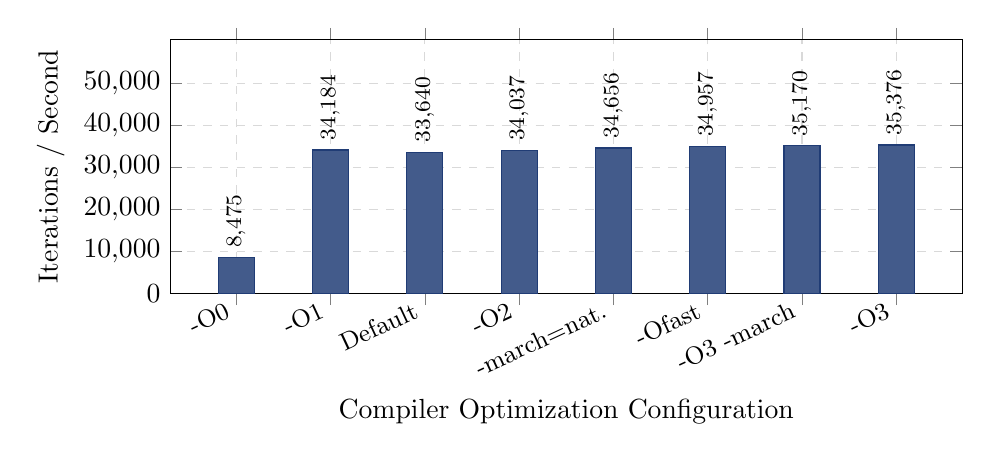
\begin{tikzpicture}
\begin{axis}[
    ybar,
    bar width=13pt,
    width=0.96\textwidth,
    height=4.8cm,
    ymin=0,
    ymax=55000,
    scaled y ticks=false,
    ytick={0, 10000, 20000, 30000, 40000, 50000},
    ylabel={Iterations / Second},
    xlabel={Compiler Optimization Configuration},
    symbolic x coords={-O0, -O1, Default, -O2, -march=nat., -Ofast, -O3 -march, -O3},
    xtick=data,
    nodes near coords,
    nodes near coords style={font=\footnotesize, rotate=90, anchor=west},
    x tick label style={rotate=25, anchor=east, font=\small},
    grid=major,
    grid style={dashed, gray!30},
    enlarge y limits={upper=0.10}
]
\addplot[fill=primaryblue!80, draw=primaryblue!95] coordinates {
    (-O0, 8475)
    (-O1, 34184)
    (Default, 33640)
    (-O2, 34037)
    (-march=nat., 34656)
    (-Ofast, 34957)
    (-O3 -march, 35170)
    (-O3, 35376)
};
\end{axis}
\end{tikzpicture}
\vspace{-0.5em}
\caption{CoreMark throughput progression across compiler optimization configurations on Apple M2. Note the massive $4.03\times$ leap between \texttt{-O0} and \texttt{-O1}, followed by fine-grained scaling plateauing at \texttt{-O3} (35,376 iter/s).}
\label{fig:performance_chart}
\end{figure}


% =========================================================================
% PAGE 3: COMPREHENSIVE COMPILER OPTIMIZATION ANALYSIS
% =========================================================================

\subsection{In-Depth Analysis of Optimization Behavior}
A rigorous evaluation of the compiler transformations explains the observed throughput variations:

\begin{enumerate}[leftmargin=1.4em]
    \item \textbf{The Memory-Bound Penalty of Unoptimized Code (\texttt{-O0}):}
    At \texttt{-O0}, Clang disables all optimization passes. Every intermediate C variable is assigned a slot in the stack frame. Across every statement, operands are read from memory via explicit load instructions (\texttt{LDR}) and written back via store instructions (\texttt{STR}). Even when variables are reused across consecutive lines, no register allocation occurs. This overwhelms the L1 data cache load/store execution pipelines and saturates store-to-load forwarding buffers. Consequently, the CPU spends the vast majority of clock cycles waiting for memory hazards and pipeline stalls, yielding only \textbf{8,474.61 iter/s} (2.43 CoreMark/MHz).

    \item \textbf{The $4.03\times$ Quantum Leap at \texttt{-O1} (Register Allocation and SSA Form):}
    Enabling \texttt{-O1} activates Static Single Assignment (SSA) construction, dead-code elimination (DCE), common subexpression elimination (CSE), and graph-coloring register allocation. By retaining loop induction variables, matrix accumulators, and list pointers within the 31 available 64-bit general-purpose ARM registers (\texttt{X0}--\texttt{X30}), memory traffic is drastically eliminated. The execution profile shifts from memory-bound to compute-bound, resulting in a dramatic \textbf{$303\%$ throughput increase} to \textbf{34,183.66 iter/s}.

    \item \textbf{The Optimization Plateau between \texttt{-O1} and \texttt{-O2}:}
    Standard compiler folklore suggests that \texttt{-O2} produces substantial speedups over \texttt{-O1}. However, our data indicates that \texttt{-O2} (\textbf{34,037.43 iter/s}) performs on par with \texttt{-O1}. This occurs because CoreMark's kernels are intentionally compact:
    \begin{itemize}
        \item The linked list traversal is governed by pointer chasing and cache latency, which cannot be vectorized or reordered.
        \item The $9\times 9$ matrix multiplication ($81$ elements) easily fits in registers; once basic loop-invariant code motion and register allocation are applied by \texttt{-O1}, standard \texttt{-O2} inlining provides marginal additional benefit.
    \end{itemize}

    \item \textbf{Peak Throughput at \texttt{-O3} (Loop Unrolling and Instruction-Level Parallelism):}
    The highest performance across all configurations is achieved by \texttt{-O3} at \textbf{35,376.00 iter/s} ($4.17\times$ speedup over \texttt{-O0}). Under \texttt{-O3}, Clang applies aggressive loop unrolling and software pipelining. In \texttt{core\_matrix.c}, unrolling the inner multiply-accumulate loop amortizes loop branch overhead, reduces counter decrement operations, and exposes independent operations that fully saturate the 8-wide out-of-order execution engine of the Apple M2.

    \item \textbf{Behavior of \texttt{-Ofast}:}
    The \texttt{-Ofast} flag enables all \texttt{-O3} optimizations along with \texttt{-ffast-math}, which relaxes strict IEEE 754 floating-point compliance (e.g., permitting reciprocal approximations and ignoring NaN/signed zeros). Because CoreMark is strictly an \textbf{integer-only benchmark}, floating-point relaxations offer zero algorithmic benefit. The recorded throughput (\textbf{34,957.08 iter/s}) is practically equivalent to \texttt{-O3}, with slight variations attributable to background OS scheduling.
\end{enumerate}

\clearpage
\begin{enumerate}[leftmargin=1.4em, start=6]
    \item \textbf{Host Architecture Tuning via \texttt{-march=native}:}
    Specifying \texttt{-march=native} instructs LLVM to generate code tailored to the host Apple M2 instruction pipeline (leveraging ARMv8.5-A scheduling models). When applied alongside base \texttt{-O2}, it produces \textbf{34,655.81 iter/s} with the \textbf{lowest variance ($\sigma = 157.83$)} among all optimized runs, proving that microarchitecture-specific instruction alignment minimizes branch target buffer (BTB) conflicts and pipeline bubbles.

    \item \textbf{CoreMark/MHz Microarchitectural Efficiency Analysis:}
    Normalizing throughput against clock frequency provides an architectural figure of merit:
    \begin{equation}
        \text{CoreMark/MHz} = \frac{\text{Mean Iterations/Sec}}{\text{Clock Frequency (MHz)}} = \frac{35376.00}{3492\text{ MHz}} = \mathbf{10.13\text{ CoreMark/MHz}}
    \end{equation}
    For comparison, embedded in-order RISC-V cores (such as RV32IMC) typically achieve \textbf{2.5--3.5 CoreMark/MHz}, while high-performance out-of-order cores reach \textbf{5.0--7.0 CoreMark/MHz}. The Apple M2 core's score of \textbf{10.13 CoreMark/MHz} underscores the exceptional instruction-level parallelism, massive out-of-order reorder buffer, and memory bandwidth of Apple Silicon.
\end{enumerate}


% =========================================================================
% PAGE 4: KEY ALGORITHMS IMPLEMENTED IN COREMARK
% =========================================================================

\section{Key Algorithms Implemented in CoreMark}
To evaluate CPU cores without distortion from standard C library implementations, CoreMark self-contains four fundamental integer algorithms (detailed in the EEMBC CoreMark specification and \textit{README.md}):

\subsection{Linked List Processing (\texttt{core\_list\_join.c})}
\begin{itemize}[leftmargin=1.4em]
    \item \textbf{Structure and Data Representation:}
    The algorithm utilizes a two-level indirect data structure:
    \begin{lstlisting}[language=C, basicstyle=\ttfamily\footnotesize, backgroundcolor=\color{lightgray}, frame=single, rulecolor=\color{bordergray}]
typedef struct list_data_s { ee_s16 data16; ee_s16 idx; } list_data;
typedef struct list_head_s {
    struct list_head_s *next;
    struct list_data_s *info;
} list_head;
    \end{lstlisting}
    Crucially, dynamic memory allocation (\texttt{malloc}) is avoided; the list resides in a pre-allocated static workspace. To model realistic heap fragmentation, \textbf{25\% of the pointers are sequential in memory}, while \textbf{75\% are non-sequential and scattered}.

    \item \textbf{Operations Executed:}
    \begin{enumerate}
        \item \textit{Find / Linear Traversal:} Executes sequential search operations seeking target values, traversing the pointer chain and feeding results into the output checksum.
        \item \textit{Merge Sort by Data:} Executes an in-place merge sort based on \texttt{data16}, and computes a 16-bit CRC checksum across the sorted sequence.
        \item \textit{Order Restoration Merge Sort:} Executes a second merge sort based on \texttt{idx}, restoring the list to its exact initial topological state for \textbf{algorithmic idempotence}.
    \end{enumerate}

    \item \textbf{Microarchitectural Stresses:}
    Exercises pointer chasing with two levels of indirection (\texttt{list\_head} to \texttt{info} to \texttt{data16}), directly exposing L1 data cache miss latency, load-to-use pipeline stalls, and branch prediction during merge sort comparisons.
\end{itemize}

\subsection{Matrix Manipulation (\texttt{core\_matrix.c})}
\begin{itemize}[leftmargin=1.4em]
    \item \textbf{Data Space Partitioning:}
    The 2000-byte workspace is partitioned equally across the three core algorithms (${\sim}666$ bytes each). For matrix manipulation, this slice allocates three $N\times N$ matrices ($N=9$): input matrices $A$ and $B$ composed of 16-bit signed integers (\texttt{ee\_s16}, 2 bytes/element) and result matrix $C$ composed of 32-bit signed integers (\texttt{ee\_s32}, 4 bytes/element), occupying exactly $81 \times (2 + 2 + 4) = 648$ bytes.
    \item \textbf{Computational Phases:}
    \begin{enumerate}
        \item Multiplication of Matrix $A$ by a runtime scalar constant $k$ into Matrix $C$.
        \item Multiplication of Matrix $A$ by a column vector from Matrix $B$ into Matrix $C$.
        \item Full Matrix-Matrix Multiply ($A \times B \to C$) via triply nested loops ($C_{i,j} = \sum_{k=0}^{N-1} A_{i,k} \cdot B_{k,j}$).
    \end{enumerate}
    The upper bits of result elements are accumulated into the runtime CRC chain.
    \item \textbf{Microarchitectural Stresses:}
    Heavily stresses \textbf{integer multiplication throughput}, multiply-accumulate (MAC) pipeline depth, strided memory access patterns, and compiler loop unrolling.
\end{itemize}

\clearpage
\subsection{Deterministic Moore State Machine (\texttt{core\_state.c})}
\begin{itemize}[leftmargin=1.4em]
    \item \textbf{Operation and Architecture:}
    A deterministic Moore state machine parses comma-separated input tokens classifying them into format categories: integers, floating-point representations, scientific notation, or invalid inputs. EEMBC explicitly selected a Moore model over a Mealy model because Mealy machines are table-driven (testing load/store operations), whereas Moore machines rely on nested conditional branches (\texttt{if-else}) and multi-way branch dispatch tables (\texttt{switch}).
    \item \textbf{Microarchitectural Stresses:}
    Stresses branch direction predictors, branch target buffers (BTB), and evaluates pipeline flush penalties resulting from mispredicted branches on pseudo-random token inputs.
\end{itemize}

\subsection{CRC Validation and Anti-Optimization Barrier (\texttt{core\_util.c})}
\begin{itemize}[leftmargin=1.4em]
    \item \textbf{Dual Architectural Purpose:}
    \begin{enumerate}
        \item \textit{Algorithmic Verification:} Verifies mathematical correctness across all iterations using 16-bit CRC checksums.
        \item \textit{Anti-Optimization Barrier:} Modern optimizing compilers eliminate dead code when results are unused. CoreMark prevents dead-code elimination by chaining intermediate results from all kernels into a volatile CRC accumulator, forcing full execution.
    \end{enumerate}
\end{itemize}


% =========================================================================
% PAGE 5: RISC-V INSTRUCTION SET ARCHITECTURE EXTENSIONS
% =========================================================================

\section{RISC-V Instruction Set Architecture (ISA) Extension Sets}
In Lab 2, CoreMark will be deployed and profiled on the configurable \textbf{CORE-V Wally processor}. Wally is an open-source, highly parameterized 5-stage / multi-stage pipelined RISC-V CPU core. Understanding the target RISC-V ISA extensions is essential for anticipating performance trends across microarchitectural configurations:

\subsection{RV32I: Base 32-bit Integer Instruction Set}
\begin{itemize}[leftmargin=1.4em]
    \item \textbf{Architectural Foundation:} The mandatory base RISC-V integer standard. It defines 32 general-purpose 32-bit registers (\texttt{x0}--\texttt{x31}, where \texttt{x0} is hardwired to zero), a 32-bit program counter, and fixed-width 32-bit instructions.
    \item \textbf{Instruction Set Repertoire (40 Base Instructions, 47 with Zicsr/Zifencei):}
    \begin{itemize}
        \item R-Type (Register-Register ALU): \texttt{ADD}, \texttt{SUB}, \texttt{SLL}, \texttt{SLT}, \texttt{SLTU}, \texttt{XOR}, \texttt{SRL}, \texttt{SRA}, \texttt{OR}, \texttt{AND}.
        \item I-Type (Immediate ALU, Loads, Jumps): \texttt{ADDI}, \texttt{SLTI}, \texttt{SLTIU}, \texttt{XORI}, \texttt{ORI}, \texttt{ANDI}, \texttt{SLLI}, \texttt{SRLI}, \texttt{SRAI}, \texttt{LB}, \texttt{LH}, \texttt{LW}, \texttt{LBU}, \texttt{LHU}, \texttt{JALR}.
        \item S-Type (Stores): \texttt{SB}, \texttt{SH}, \texttt{SW}.
        \item B-Type (Conditional Branches): \texttt{BEQ}, \texttt{BNE}, \texttt{BLT}, \texttt{BGE}, \texttt{BLTU}, \texttt{BGEU}.
        \item U-Type (Upper Immediates): \texttt{LUI}, \texttt{AUIPC}.
        \item J-Type (Unconditional Jumps): \texttt{JAL}.
        \item System / Environment: \texttt{ECALL}, \texttt{EBREAK}, \texttt{FENCE}. (Under the modern unprivileged RISC-V specification, CSR access instructions are modularized into the \textbf{Zicsr} extension and instruction synchronization into \textbf{Zifencei}, yielding 40 unprivileged base instructions or 47 when bundled with CSR/fence extensions).
    \end{itemize}
    \item \textbf{Critical CoreMark Implication:} \textbf{RV32I possesses no hardware multiplier or divider.} All integer multiplications in \texttt{core\_matrix.c} (matrix dot products, scalar scalings) must be emulated in software via compiler runtime routines (\texttt{\_\_mulsi3}), which execute 30--40 shift-and-add instructions per multiply. This imposes a severe computational bottleneck on pure RV32I. (In contrast, CRC calculation in \texttt{core\_util.c} relies solely on logical shifts, XOR, and bitwise masking, requiring no hardware multiplier).
\end{itemize}

\clearpage
\subsection{RV32IM: Standard Extension for Integer Multiplication and Division}
\begin{itemize}[leftmargin=1.4em]
    \item \textbf{Hardware Enhancement:} Adds dedicated hardware multiplier and divider execution blocks in the ALU stage.
    \item \textbf{Added Instructions (8 Instructions):}
    \begin{itemize}
        \item Multiplication: \texttt{MUL} (lower 32 bits), \texttt{MULH} (signed high 32 bits), \texttt{MULHU} (unsigned high 32 bits), \texttt{MULHSU} (signed-unsigned high 32 bits).
        \item Division and Remainder: \texttt{DIV}, \texttt{DIVU}, \texttt{REM}, \texttt{REMU}.
    \end{itemize}
    \item \textbf{CoreMark Impact:} Delivers the \textbf{single largest performance acceleration} in the benchmark suite. In \texttt{core\_matrix.c}, the triple-nested loop performs $N^3$ multiplications. Replacing ${\sim}35$-cycle software emulation loops with 1- to 3-cycle pipelined hardware \texttt{MUL} instructions yields an anticipated $3\times$ to $6\times$ throughput improvement over RV32I.
\end{itemize}

\subsection{RV32IMC: Standard Extension for Compressed Instructions}
\begin{itemize}[leftmargin=1.4em]
    \item \textbf{Architectural Foundation:} Adds 16-bit compressed instruction encodings that interleave freely with standard 32-bit instructions on any 16-bit aligned boundary (e.g., \texttt{C.LW}, \texttt{C.SW}, \texttt{C.ADD}, \texttt{C.J}, \texttt{C.BEQZ}).
    \item \textbf{Code Density:} Compresses compiled binary footprint by \textbf{25\% to 35\%}.
    \item \textbf{CoreMark Impact:} By significantly shrinking the static loop footprints, the C extension drastically improves \textbf{Instruction Cache (I-cache) hit rates}. On cache-constrained embedded processors such as Wally, fewer fetch cycles are wasted waiting for main memory or bus transfers, yielding substantial throughput gains.
\end{itemize}

\subsection{RV32GC: General-Purpose ISA Standard}
\begin{itemize}[leftmargin=1.4em]
    \item \textbf{Architectural Definition:} The standard ``G'' bundle represents the full general-purpose platform:
    \begin{equation}
        \mathbf{G} = \mathbf{I} + \mathbf{M} + \mathbf{A} + \mathbf{F} + \mathbf{D} + \mathbf{Zicsr} + \mathbf{Zifencei}
    \end{equation}
    Combined with \textbf{C}, RV32GC represents the baseline hardware profile capable of hosting rich operating systems like Linux.
    \item \textbf{Constituent Extensions:}
    \begin{itemize}
        \item \textbf{A (Atomic):} Adds load-reserved/store-conditional (\texttt{LR.W}/\texttt{SC.W}) and atomic memory operations (\texttt{AMO*}) for multi-core thread synchronization.
        \item \textbf{F \& D (Floating-Point):} Single- and double-precision IEEE 754 coprocessors with 32 dedicated floating-point registers (\texttt{f0}--\texttt{f31}) and the \texttt{fcsr} status register.
    \end{itemize}
    \item \textbf{CoreMark Impact:} CoreMark's integer kernels do not invoke floating-point instructions; however, the 'A' extension enables multi-threaded CoreMark configurations (\texttt{-DMULTITHREAD=N}), permitting linear performance scaling across multiple cores.
\end{itemize}

\subsection{RV64I: Base 64-bit Integer Instruction Set}
\begin{itemize}[leftmargin=1.4em]
    \item \textbf{Architectural Foundation:} Expands the integer register file and datapath to \textbf{XLEN = 64 bits}.
    \item \textbf{Instruction Set Additions:} Adds 64-bit load/store instructions (\texttt{LD}, \texttt{SD}) and word-specific instructions operating on 32-bit sub-words with sign-extension (e.g., \texttt{ADDIW}, \texttt{ADDW}, \texttt{SUBW}, \texttt{SLLW}, \texttt{SRLW}, \texttt{SRAW}, \texttt{LWU}).
    \item \textbf{CoreMark Trade-Offs:} While 64-bit registers enable single-cycle 64-bit arithmetic, pointers double in size from 4 bytes to 8 bytes. In \texttt{core\_list\_join.c}, this increases cache line footprint and L1D cache pressure compared to RV32.
\end{itemize}


% =========================================================================
% PAGE 6: ARCHITECTURAL SYNTHESIS AND CONCLUSION
% =========================================================================

\clearpage
\section{Comparative Synthesis and Projections for CORE-V Wally (Lab 2)}

\subsection{Architectural Comparison Matrix}
Table~\ref{tab:riscv_synthesis} synthesizes the architectural characteristics and expected CoreMark performance profiles across the evaluated RISC-V ISA configurations.

\begin{table}[H]
\centering
\small
\caption{Comprehensive RISC-V ISA Architectural Comparison for CORE-V Wally}
\label{tab:riscv_synthesis}
\resizebox{\textwidth}{!}{%
\begin{tabular}{l c c c c c}
\toprule
\textbf{Architectural Metric} & \textbf{RV32I} & \textbf{RV32IM} & \textbf{RV32IMC} & \textbf{RV32GC} & \textbf{RV64I} \\
\midrule
\textbf{Register File Width (XLEN)} & 32 bits & 32 bits & 32 bits & 32 bits (Int) + 64 bits (FP) & 64 bits \\
\textbf{Hardware Multiplier/Divider} & None (Emulated) & Dedicated Pipelined Unit & Dedicated Pipelined Unit & Dedicated Pipelined Unit & None (Emulated) \\
\textbf{Compressed Encoding Support} & No (32-bit only) & No (32-bit only) & Yes (16/32-bit mixed) & Yes (16/32-bit mixed) & No (32-bit only) \\
\textbf{Floating-Point Coprocessor} & None & None & None & Single (F) \& Double (D) & None \\
\textbf{Relative Code Size} & $1.00\times$ (Baseline) & $\approx 0.98\times$ & $\mathbf{\approx 0.70\times}$ & $\approx 0.72\times$ & $\approx 1.05\times\text{--}1.10\times$ (64-bit Immediates) \\
\textbf{Expected CoreMark Relative to RV32I} & $1.00\times$ (Baseline) & $\mathbf{3.5\times\text{--}5.5\times}$ & $\mathbf{4.0\times\text{--}6.2\times}$ & $4.0\times\text{--}6.2\times$ (Single-Core) & $0.95\times\text{--}1.10\times$ \\
\textbf{Primary Pipeline Bottleneck} & Software \texttt{\_\_mulsi3} & Memory / Branch stalls & Instruction fetch stalls & FPU silicon unutilized & L1D pressure (8B pointers) \\
\bottomrule
\end{tabular}%
}
\end{table}

\subsection{Empirical Hypotheses for Lab 2 Simulation}
Based on our host profiling and architectural analysis, we formulate the following testable hypotheses for Lab 2 on CORE-V Wally:
\begin{enumerate}[leftmargin=1.4em]
    \item \textbf{Hypothesis 1 (The Hardware Multiplier Acceleration):} Upgrading from RV32I to RV32IM will yield a massive jump ($>3.5\times$) in CoreMark throughput. In \texttt{core\_matrix.c}, the triple-nested loops execute tens of thousands of multiplications. Hardware \texttt{MUL} execution eliminates thousands of software emulation instructions.
    \item \textbf{Hypothesis 2 (Instruction Cache Benefits of Compressed Instructions):} Enabling the C extension (RV32IMC) will reduce binary size by ${\sim}30\%$, significantly increasing instruction cache hit rates in Wally's tightly constrained I-cache. This will translate to a measurable $10\%\text{--}20\%$ performance boost over RV32IM.
    \item \textbf{Hypothesis 3 (Neutral Impact of F and D in Single-Threaded CoreMark):} Profiling RV32GC against RV32IMC will reveal nearly identical single-thread CoreMark throughput because CoreMark contains no floating-point kernels. However, RV32GC incurs greater silicon area overhead.
    \item \textbf{Hypothesis 4 (Pointer Overhead in RV64I):} Comparing RV64I to RV32I will demonstrate that 64-bit architectures without hardware multiplication suffer slightly higher data cache pressure due to 8-byte pointer storage in \texttt{core\_list\_join.c}.
\end{enumerate}

\section{Conclusion}
This prelab investigation established a rigorous empirical and architectural baseline for processor benchmarking:
\begin{enumerate}[leftmargin=1.4em]
    \item \textbf{Compiler Optimization Impact:} On the host Apple M2, compiler optimization levels produce a $\mathbf{4.17\times}$ throughput expansion (from 8,474.61 iter/s at \texttt{-O0} to 35,376.00 iter/s at \texttt{-O3}). The primary gain ($4.03\times$) occurs at \texttt{-O1} through SSA-based register allocation, with incremental gains at \texttt{-O3} driven by loop unrolling.
    \item \textbf{Microarchitectural Efficiency:} Normalizing host performance against the 3.49 GHz clock frequency yields an outstanding score of $\mathbf{10.13\text{ CoreMark/MHz}}$, reflecting the high instruction-level parallelism of Apple Silicon.
    \item \textbf{Algorithmic Diversity:} CoreMark's four kernels comprehensively stress key CPU subsystems: pointer chasing and data cache latency (linked list), ALU multiplication and register pressure (matrix), branch prediction and pipeline flush penalties (Moore state machine), and algorithmic execution integrity (CRC).
    \item \textbf{Preparedness for Lab 2:} The theoretical foundation established in this report directly equips us to profile, evaluate, and interpret architectural trade-offs across RV32I, RV32IM, RV32IMC, RV32GC, and RV64I on the CORE-V Wally processor.
\end{enumerate}

\end{document}
